\chapter{Architektura a implementace aplikace}

\begin{figure}
	\centering
	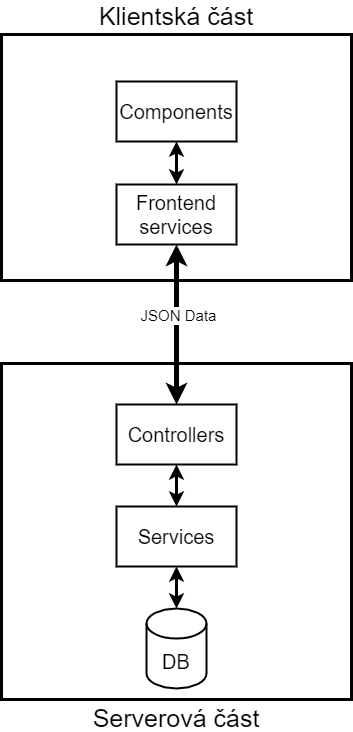
\includegraphics[height=0.5\textheight]{architecture.PNG}
	\caption{Architektura aplikace}
	\label{fig:Architecture}
\end{figure}

Aplikace se skládá ze 2 hlavních částí: serverové a klientské.

Na obrázku \ref{fig:Architecture} vidíme architekturu aplikace, šipky znázorňují přenos dat. Jednotlivým částem se budeme podrobněji věnovat v této kapitole.

\section{Serverová část}

Serverová část aplikace je naprogramovaná v jazyce C\# s použitím 
frame\-worku ASP .NET Core. Je rozdělena do těchto projektů:

\begin{itemize}
	\item Data
	\item Services
	\item API
	\item TestEvaluation
	\item TestEvaluation.Tests
\end{itemize}

\subsection{Data}

Tento projekt se stará primárně o komunikaci s databází, pro tento účel jsme použili ORM framework Entity Framework Core. 

Ve složce \textit{Models} jsou třídy reprezentující databázové entity. Každá z entit pak v databázi představuje jednu tabulku. V aplikaci jsme použili tyto entity, vztahy mezi nimi můžeme vidět na obrázku \ref{fig:DbModel}.

\begin{table}[ht]
	\centering
	\begin{tabular}{| l | p{9cm} |}
		\hline
		Název entity & reprezentovaný objekt \\
		\hline \hline
		Course & kurz \\ \hline
		CourseAdmin & vztah administrátor mezi entitami Course a Person \\ \hline		
		CourseFile & nějaký soubor sdílený v kurzu \\ \hline
		CourseMember & členství uživatele v daném kurzu. 
		K této entitě se pak vážou všechny známky a odeslané testy. \\ \hline
		CourseTest & test v kurzu. Testy dělíme na hodnocené a nehodnocené (tzv. kvízy). \\ \hline
		EnrollmentRequest & žádost o zapsání uživatele do daného kurzu \\ \hline
		ForumPost & příspěvek ve fóru k danému kurzu \\ \hline
		Grade & známku kterou student obdržel (kromě známek z testů) \\ \hline
		Person & uživatele aplikace \\ \hline
		TestQuestion & jednu otázku v testu \\ \hline
		TestSubmission & test s odpověďmi odeslaný uživatelem \\ \hline
		TestSubmissionAnswer & odpověď k dané otázce v testu \\
		\hline
	\end{tabular}
\end{table}

\newpage

\begin{figure}
	\centering
	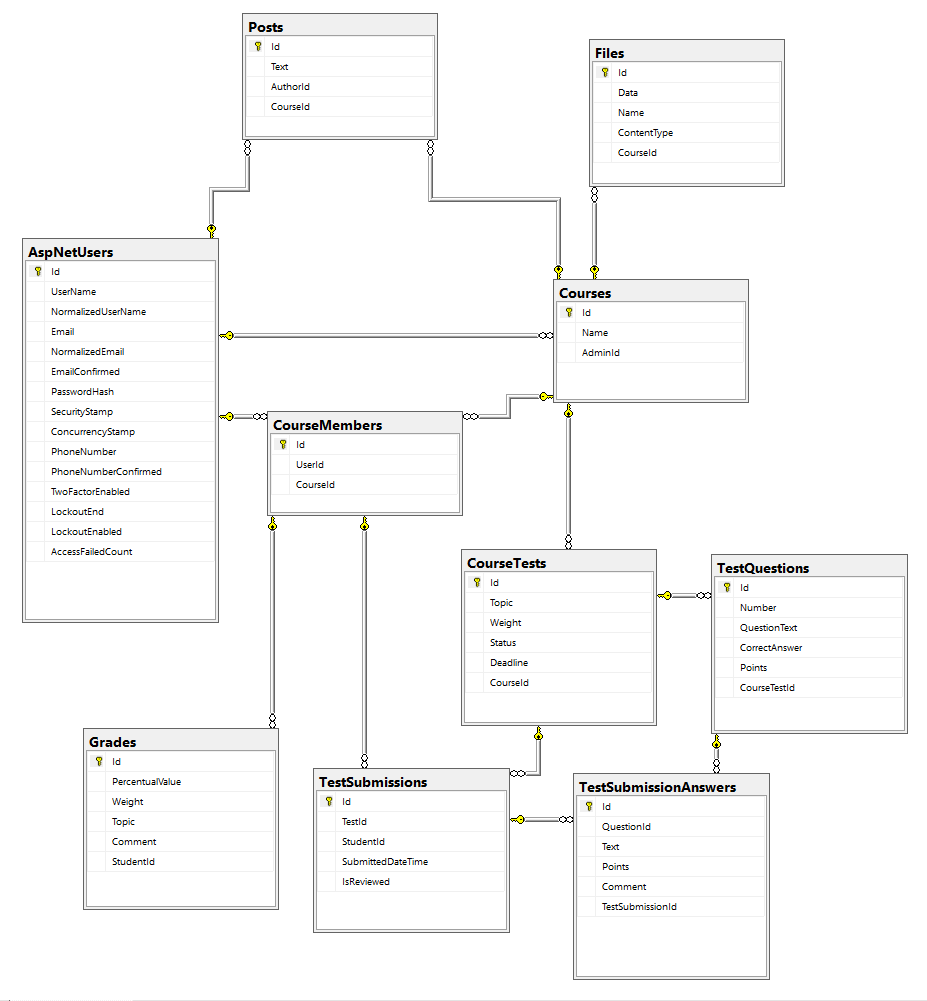
\includegraphics[width=\textwidth]{db_model.PNG}
	\caption{Databázový model aplikace}
	\label{fig:DbModel}
\end{figure}

\newpage

Pro ilustraci uvedeme kód třídy \textit{Course} (Kód \ref{CourseClass}).

\begin{program}
	\begin{lstlisting}
	public class Course : IGuidIdObject
	{
		public Course()
		{
			Members = new List<CourseMember>();
			Files = new List<CourseFile>();
			Tests = new List<CourseTest>();
			...
		}
		
		public Course(string name, Person admin) : this()
		{
			Name = name;
			Admin = admin;
		}
		
		/// <summary>
		/// identifier of the couse
		/// </summary>
		[DatabaseGenerated(DatabaseGeneratedOption.Identity)]
		[Key]
		public Guid Id { get; set; }
		
		/// <summary>
		/// name of the course
		/// </summary>
		[Required]
		public string Name { get; set; }
		
		...
	\end{lstlisting}
	\caption{Ukázka třídy \textit{Course}}
	\label{CourseClass}
\end{program}

Vidíme, že každá entita obsahuje veřejné vlastnosti (public properties) s gettery a settery. Tyto vlastnosti budou v databázové tabulce reprezentovány jako sloupce. Některé z nich (jako např. \textit{Id}) obsahují ještě doplňující atributy, ty slouží k upřesnění informací o dané vlastnosti. Například atribut \textit{[Key]} určuje, že tato vlastnost bude v databázi primární klíč, atribut \textit{[Required]} určuje, že daný sloupec bude v tabulce u všech záznamů povinný (tedy hodnoty budou \textit{NOT NULL}).
Dále musí každá entita obsahovat konstruktor bez parametrů.

Vazby mezi entitami jsou reprezentované pomocí tzv. navigačních vlastností. V případě, že chceme vytvořit vazbu typu one-to-many mezi entitami A a B, stačí do vlastností třídy A přidat kolekci objektů typu B, a naopak do třídy B vlastnost typu A. Framework pak při provádění migrace vytvoří v databázové tabulce entity B vytvoří sloupec s cizím klíčem, který bude obsahovat identifikátor entity A, ke které patří.

V aplikaci je vazba one-to-many použita mimo jiné mezi entitami \textit{Course} a \textit{CourseTest}, a to tak, že každý test je obsažen v právě jednom kurzu, a v daném kurzu může být N testů.
Kód pak tedy vypadá takto: Ve třídě \textit{Course} je kolekce objektů typu \textit{CourseTest}

\begin{lstlisting}
/// <summary>
/// tests in this course
/// </summary>
public ICollection<CourseTest> Tests { get; set; }
\end{lstlisting}

Ve třídě \textit{CourseTest} je pak vlastnost typu \textit{Course}

\begin{lstlisting}
/// <summary>
/// course that contains this test
/// </summary>
[Required]
public Course Course { get; set; }
\end{lstlisting}

Po provedení databázové migrace (viz. dále) se v tabulce \textit{CourseTest} vytvoří sloupec \textit{CourseId} s cizím klíčem, který odkazuje na identifikátor kurzu (tzn. vlastnost \textit{Course.Id}).

Také si můžeme všimnout, že všechny entity (kromě entity \textit{Person}) implementují rozhraní IGuidObject. To je jednoduché rozhraní, které obsahuje pouze jednu vlastnost -- \textit{Id} typu \textit{Guid}. Tímto máme zajištěnou jednotu identifikátorů, tedy že všechny entity, které toto rozhraní implementují, budou mít identifikátor typu \textit{Guid}.

\begin{lstlisting}
/// <summary>
/// interface for object with <see cref="Guid"/> identifier
/// </summary>
public interface IGuidIdObject
{
	/// <summary>
	/// identifier of the object
	/// </summary>
	Guid Id { get; set; }
}
\end{lstlisting}


Typ \textit{Guid} jsme zvolili hlavně z toho důvodu, že vestavěné tabulky frameworku (např. \textit{Identity}) mají také řetězcové identifikátory. Navíc se pak zjednoduší práce ve frontend části (není potřeba parsovat \textit{string} na \textit{int} např. v klientské části při práci s URL). Tyto identifikátory generuje databáze, takže je zajištěno, že jsou unikátní.
Další možnost by byla použít jako identifikátor číslo (např. typ \textit{int}), ale vzhledem k výše uvedeným argumentům je typ \textit{Guid} v tomto případě lepší možnost.

Dále se v projektu nacházejí také rozhraní \textit{ICourseReferenceObject} a \textit{ICourseMemberReferenceObject}, která slouží k tomu, abychom mohli dále v aplikaci jednotně pracovat s objekty, které mají referenci na entitu \textit{Course}, resp. \textit{CourseMember}. Tato rozhraní implementují pouze nějaké entity.

Třída \textit{CMSDbContext} reprezentuje databázový kontext této aplikace. Každý objekt typu \textit{DbSet} pak představuje jednu databázovou tabulku. Ve třídě \textit{CMSDbContext} je tedy kolekce typu \textit{DbSet} pro každou z entit.

\begin{lstlisting}
public DbSet<Grade> Grades { get; set; }

public DbSet<Course> Courses { get; set; }

...
\end{lstlisting}

Jediná výjimka je entita \textit{Person}, která dědí ze třídy \textit{IdentityUser}, a jejíž \textit{DbSet} je nakonfigurovaný ve frameworku. 

V programu pak dále používáme ke komunikaci s databází pouze třídu \textit{CMSDbContext} a objekty typu \textit{DbSet}. Třída \textit{DbSet<TEntity>} implementuje rozhraní \textit{IQueryable<TEntity>}, takže na ni lze použít LINQ. Pokud bychom chtěli například vybrat všechny kurzy, jejichž jméno začíná na písmeno C, pak stačí použít následující LINQ dotaz
\begin{lstlisting}
dbContext.Courses.Where(course => course.Name.StartsWith("C"))
\end{lstlisting}
kde proměnná \textit{dbContext} je instance třídy \textit{CMSDbContext}.

Ve třídě \textit{CMSDbContext} je také metoda \textit{ConfigureForeignKeys}, která provede konfiguraci cizích klíčů v aplikaci. Všechny políčka s cizími klíči jsou v databázi povinné (tzn. \textit{NOT NULL}), to je zajištěno pomocí atributu \textit{[Required]} daných vlastností. Nastavením \textit{DeleteBehavior.Restrict} u cizích klíčů zajistíme, že databáze zůstane v konzistentním stavu. Pokud bychom tedy chtěli smazat entitu, pak na ni nesmí pomocí cizích klíčů odkazovat jiné entity. V opačném případě program při zavolání metody \textit{SaveChanges()} na databázovém kontextu vyhodí výjimku.

V programu je dále složka \textit{Migrations}. Při vývoji byl použit princip Code first, tedy že v kódu specifikujeme entity pomocí klasických tříd. Framework se pak postará o vytvoření databázových tabulek z tohoto kódu.

Pokud tedy nějak změníme některou z entit (to může být např. přidání vlastnosti, změna jména vlastnosti, apod.), pak pomocí ORM můžeme vygenerovat soubor popisující tzv. databázovou migraci, která slouží k aplikaci změn z kódu do databáze. Ke každé migraci se vygeneruje jeden soubor, který obsahuje popis změn, které se později provedou v databázi.

K vytváření migrací jsem použijeme nástroj CLI tools for Entity Framework Core. \cite{EfCoreCliDocs} Pro vygenerování migrace ze změn v kódu použijeme příkaz:

\begin{lstlisting}
dotnet ef migrations add 
\end{lstlisting}

Tímto se vytvoří soubor popisující změny v migraci, ale databáze zatím zůstala beze změny. Tento soubor obsahuje třídu, jenž dědí ze třídy \textit{Migration} a obsahuje metody \textit{Up} a \textit{Down}. V metodě \textit{Up} je popis změn, které se provedou při aplikaci této migrace, naopak v metodě \textit{Down} je popis změn, které se provedou v případě odstranění migrace.

Jako příklad si můžeme představit migraci, která obsahuje přidání vlastnosti \textit{ScoreWeight} k entitě \textit{CourseTest} (tato vlastnost popisuje váhu testu).
Vygenerovaný kód migrace pak můžeme vidět v ukázce kódu \ref{MigrationExample}.

\begin{program}
	\begin{lstlisting}
	public partial class TestWeight_added : Migration
	{
		protected override void Up(MigrationBuilder migrationBuilder)
		{
			migrationBuilder.AddColumn<int>(
			name: "ScoreWeight",
			table: "CourseTests",
			nullable: false,
			defaultValue: 0);
		}
		
		protected override void Down(MigrationBuilder migrationBuilder)
		{
			migrationBuilder.DropColumn(
			name: "ScoreWeight",
			table: "CourseTests");
		}
	}
	\end{lstlisting}
	\caption{Příklad migrace}
	\label{MigrationExample}
\end{program}

Pro promítnutí změn do databáze následně použijeme příkaz:

\begin{lstlisting}
dotnet ef database update
\end{lstlisting}

Tímto tedy dojde k změnám v databázi (v našem příkladu se vytvoří sloupec \textit{ScoreWeight} v tabulce \textit{CourseTests}).

V obou příkazech je potřeba specifikovat cílový a startup projekt. Cílový projekt je ten, který obsahuje databázový kontext a entity naší aplikace (v tomto případě projekt Data). Naopak startup projekt je projekt, který je spouštěný frameworkem, což je potřeba pro získání konfiguračních informací o projektu, jako je například connection string do naší databáze.

\subsection{Services}
V tomto projektu se nachází pomocné služby pro komunikaci s databází. 

Jako základ pro všechny služby slouží abstraktní třída \textit{DbService} (Kód \ref{DbService}), která obsahuje referenci na databázový kontext aplikace a jedinou metodu \textit{CommitChanges()}. Ta slouží k uložení změn provedených v databázovém kontextu do databáze. 

To je potřeba, protože k uložení změn do databáze dojde až tehdy, když na databázovém kontextu zavoláme metodu \textit{SaveChanges()}. Pokud bychom tedy například do databázového kontextu něco uložili (např. takto: 
\begin{lstlisting}
dbContext.Grades.Add(new Grade())
\end{lstlisting})
a nezavolali metodu \textit{dbContext.SaveChanges()}, data by se neuložila.

\begin{program}
	\begin{lstlisting}
	/// <summary>
	/// class representing base database service
	/// </summary>
	public abstract class DbService : IDbService
	{
		/// <summary>
		/// context of the CMS database
		/// </summary>
		protected readonly CMSDbContext dbContext;
		
		protected DbService(CMSDbContext dbContext)
		{
			this.dbContext = dbContext;
		}
		
		/// <inheritdoc/>
		public void CommitChanges()
		{
			dbContext.SaveChanges();
		}
	}
	\end{lstlisting}
	\caption{Třída \textit{DbService}}
	\label{DbService}
\end{program}

Tato třída implementuje rozhraní \textit{IDbService}, které obsahuje pouze metodu \textit{CommitChanges()}.

Dále jsou ve složce \textit{Interfaces} rozhraní pro další služby, ty jsou rozdělené podle entit (typicky máme pro jednu entitu jednu službu). Všechny tyto rozhraní také implementují rozhraní \textit{IDbService}. 

Rozhraní \textit{ICourseService} (slouží pro práci s kurzy) můžeme vidět v kódu \ref{ICourseService}.
\begin{program}
	\begin{lstlisting}
	public interface ICourseService : IDbService
	{
		/// <summary>
		/// get course by its id
		/// </summary>
		/// <param name="courseId">identifier of the course</param>
		/// <returns></returns>
		Course GetById(string courseId);
		
		/// <summary>
		/// archive course by its id
		/// </summary>
		/// <param name="courseId">id of the course to delete</param>
		void ArchiveById(string courseId);
		
		/// <summary>
		/// add the course into the database
		/// </summary>
		/// <param name="course">course to add</param>
		void AddCourse(Course course);
		...
	\end{lstlisting}
	\caption{Rozhraní \textit{ICourseService}}
	\label{ICourseService}
\end{program}

Ve složce \textit{Implementations} jsou potom implementace těchto rozhraní. Můžeme vidět, že všechny implementace dědí ze třídy \textit{DbService}, a zároveň také tranzitivně implementují \textit{IDbService}.

Třídu \textit{CourseService}, která implementuje rozhraní \textit{ICourseService} můžeme vidět na ukázce kódu \ref{CourseService}.

\begin{program}
	\begin{lstlisting}
	public class CourseService : DbService, ICourseService
	{
		public CourseService(CMSDbContext dbContext) : base(dbContext)
		{ }
		
		/// <inheritdoc/>
		public void ArchiveById(string courseId)
		{
			Course c = GetById(courseId);
			c.IsArchived = true;
		}
		
		/// <inheritdoc/>
		public Course GetById(string courseId)
		{
			return dbContext.Courses.FindById(courseId);
		}
		
		/// <inheritdoc/>
		public void AddCourse(Course course)
		{
			dbContext.Courses.Add(course);
		}
		...
	\end{lstlisting}
	\caption{Třída \textit{CourseService}}
	\label{CourseService}
\end{program}

Vidíme, že služby typicky pracují s databázovým kontextem a s daty (vyhledávání, mazání, apod.).
Dále si můžeme všimnout, že v žádné metodě se neukládají změny do databáze (tzn. volání metody \textit{CommitChanges()}). To je z toho důvodu, že ve vyšších vrstvách aplikace (např. API) v jedné metodě často voláme několik služeb, příp. několik metod z jedné služby. 
Pokud bychom v metodách služeb přímo ukládali změny do databáze (metoda \textit{CommitChanges()}), pak bychom se mohli lehce dostat to nekonzistentního stavu. To například tak, že při volání několika služeb v rámci jedné metody by 
mohla některá ze služeb vyhodit výjimku, nicméně všechny služby zavolané předtím by už data uložily.

Je na zodpovědnosti volajícího provést uložení změn do databáze, tedy zavolat metodu \textit{CommitChanges()}, což je typicky poslední příkaz v dané metodě.
Tím jsme tedy zajistili konzistenci dat - buď se do databáze uloží všechny změny provedené v databázovém kontextu, nebo žádné.

Dále si můžeme všimnout, že ve službách pracujeme s identifikátory typu \textit{string}, ale v databázi používáme typ \textit{Guid}. To je z toho důvodu, že ve vyšších vrstvách aplikace se pohodlněji pracuje se stringy (např. často dostáváme ID jako URL parametr). Převod mezi typy \textit{string} a \textit{Guid} pak řešíme ve službách.

Ve složce \textit{Extensions} jsou pak pomocné metody pro práci s některými třídami.

Ve třídě \textit{DbSetExtensions} se nachází extension metody pro třídu \textit{DbSet<T>}. Vybereme si například metodu \textit{GetCourseIdOf}, ta slouží k získání ID kurzu, ke kterému daný objekt, jenž má referenci na entitu \textit{Course}, patří.
\begin{lstlisting}
public static string GetCourseIdOf<T>(this DbSet<T> dbSet, string objectId) where T : class, ICourseReferenceObject, IGuidIdObject
{
	return dbSet.Include(item => item.Course)
		.Single(item => item.Id.ToString() == objectId)
		.Course.Id.ToString();
}
\end{lstlisting}

Vidíme, že toto je jeden z příkladů použití rozhraní \textit{ICourseReferenceObject}, které se nachází v projektu Data.

V projektu též máme rozhraní \textit{ICourseReferenceService}, to implementují vše\-chny služby, jejichž entity logicky patří k nějakému kurzu. Rozhraní obsahuje jedinou metodu \textit{GetCourseIdOf(string objectId)}, která získá ID kurzu, ke kterému daná entita patří. V implementaci této metodu pak typicky používáme extension metodu \textit{GetCourseIdOf} pro třídu \textit{DbSet<T>}. Například ve třídě \textit{CourseTestService} vypadá implementace takto:

\begin{lstlisting}
public string GetCourseIdOf(string objectId)
{
	return dbContext.CourseTests.GetCourseIdOf(objectId);
}
\end{lstlisting}

Podobně je v projektu i rozhraní \textit{ICourseMemberReferenceService}, které používají služby, jejichž entity mají referenci na třídu \textit{CourseMember}.

Použitím služeb jsme odstranili duplikátní kód (např. hledání kurzu podle ID se používá na několika místech ve vyšších vrstvách), a extrahovali některé složitější dotazy do samostatných metod. To je výhodné hlavně z toho důvodu, že je pak můžeme nezávisle otestovat. Další výhoda je, že vyšší vrstvy jsou odstíněny od použití ORM (a databázového kontextu), pouze volají tyto služby.

Dále si můžeme všimnout, že ve službách používáme při komunikaci s databázovým kontextem tzv. Eager loading (pomocí metod \textit{Include()}). To znamená, že data databázových entit které daná entita referencuje, se při výchozím chování nenačtou (pokud nepoužijeme metodu \textit{Include}), tzn. budou mít hodnotu \textit{NULL}.

Například pro získání testu s otázkami můžeme použít tento příkaz:
\begin{lstlisting}
dbContext.CourseTests
	.Include(test => test.Questions)
\end{lstlisting}
Pokud bychom volání metody Include() vynechali, tak by se data otázek nenačetla.

\subsection{API}
V této části se nachází popis projektu API, které slouží pro komunikaci klientské části se serverovou.

\subsubsection*{Controllers}
Controllery slouží primárně ke zpracování HTTP požadavků. Vidíme, že Controller je klasická C\# třída, jež dědí ze třídy \textit{ControllerBase}. Ve většině případů obsahuje reference na služby (jako privátní položky). Kód \ref{CoursesController} ukazuje příklad Controlleru, který slouží k práci s kurzy.

\begin{program}
	\begin{lstlisting}
	[Route("api/[controller]")]
	[ApiController]
	[Authorize]
	public class CoursesController : ControllerBase
	{
		private readonly IHttpContextAccessor httpContextAccessor;
		private readonly ICourseService courseService;
		private readonly IPeopleService peopleService;
		private CourseTestFilter courseTestFilter;
		...
		
		public CoursesController(IHttpContextAccessor httpContextAccessor, ICourseService courseService, IPeopleService peopleService)
		{
			this.httpContextAccessor = httpContextAccessor;
			this.courseService = courseService;
			this.peopleService = peopleService;
			courseTestFilter = new CourseTestFilter();
			...
		}
		...
	\end{lstlisting}
	\caption{Ukázka třídy \textit{CoursesController}}
	\label{CoursesController}
\end{program}

Jednotlivé Controllery pak obsahují veřejné metody, jež odpovídají HTTP endpointům.

Ukázka kódu \ref{ControllerMethod1} obsahuje metodu, která slouží k získaní všech členů daného kurzu.

\begin{program}
	\begin{lstlisting}
	/// <summary>
	/// get all course members
	/// </summary>
	/// <param name="courseId">Id of the course</param>
	[HttpGet("{courseId}/members")]
	[AuthorizeCourseAdminOf(EntityType.Course, "courseId")]
	public IEnumerable<CourseMemberOrAdminVM> GetAllMembers(string courseId)
	{
		var people = courseService.GetMembersWithUsers(courseId);
		return people.Select(cm => new CourseMemberOrAdminVM(cm.Id.ToString(), cm.User.UserName, cm.User.Email));
	}
	\end{lstlisting}
	\caption{Ukázka metody Controlleru}
	\label{ControllerMethod1}
\end{program}

Vidíme, že je tedy označená atributem \textit{HttpGet}, který zároveň obsahuje URL, přes kterou lze tuto metodu zavolat. V tomto případě je URL suffix \textit{\{courseId\}/members}. Položka \textit{courseId} označuje parametr, jenž má stejnou hodnotu jako proměnná \textit{courseId} (parametr metody). Tento suffix se připojí za URL daného Controlleru, a tím získáme celou URL k zavolání této metody. V našem případě dostaneme
\newline
\textit{http://host/api/courses/course-id/members}, kde \textit{course-id} je identifikátor příslušného kurzu a host označuje URL serveru, na kterém aplikace běží. Pokud máme aplikaci spuštěnou lokálně, pak by hodnota měla být \textit{localhost:5001}. Při HTTP GET dotazu na tuto URL by tedy aplikace zavolala tuto metodu, a vrátila data ve formátu JSON.

Metoda dále obsahuje atribut určený k autorizaci, pomocí něhož ověříme, že klient má dostatečná práva. V tomto případě povolíme zavolat metodu pouze administrátorům daného kurzu.

V těle metody pak zavoláme konkrétní službu, která typicky pracuje s databází. Tato služba nám vrátí data (v tomto případě všechny členy daného kurzu), které potom namapujeme na objekty typu ViewModel, a ty vrátíme.

\vspace{\baselineskip}

V dalším příkladu (Kód \ref{ControllerMethod2}) máme metodu, která slouží k vytvoření nového kurzu.

\begin{program}
	\begin{lstlisting}
	/// <summary>
	/// create new course
	/// </summary>
	[HttpPost("create")]
	public void Create(AddCourseVM courseVM)
	{
		string currentUserId = httpContextAccessor
			.HttpContext.GetCurrentUserId();
		Person admin = peopleService.GetById(currentUserId);
		Course createdCourse = new Course(courseVM.Name, admin);
		
		courseService.AddCourse(createdCourse);
		
		courseService.CommitChanges();
	}
	\end{lstlisting}
	\caption{Ukázka metody Controlleru}
	\label{ControllerMethod2}
\end{program}

Tato metoda je označena atributem \textit{HttpPost}, který opět obsahuje URL suffix. Pokud bychom tedy chtěli zavolat tuto metodu, pak je potřeba provést HTTP POST požadavek na URL
\newline
\textit{http://host/api/courses/create}, který v těle obsahuje JSON objekt typu \textit{AddCourseVM}. Framework pak provede deserializaci objektu, a objekt (instanci třídy \textit{AddCourseVM}) předá jako parametr do této metody.

V těle metody následně vytvoříme nový objekt kurzu, a pomocí příslušné služby (v tomto případě \textit{CourseService}) jej přidáme k existujícím kurzům. Můžeme si všimnout, že na konci metody voláme metodu \textit{CommitChanges()}, která změny zapíše do databáze.

\subsubsection*{ViewModels}
\label{serverVM}

ViewModels reprezentují objekty pro komunikaci mezi Frontend a Backend částí (konkrétně mezi Frontend službami a API). Tedy např. při GET dotazu vrací příslušný Controller objekt (příp. objekty) typu ViewModel a framework automaticky provede serializaci do formátu JSON. Stejně tak při POST dotazu posílá klient v těle požadavku objekt typu ViewModel.

Příklad ViewModelu vidíme v kódu \ref{SubmitTestVM}.

\begin{program}
	\begin{lstlisting}
	/// <summary>
	/// viewmodel for submitting a test
	/// </summary>
	public class SubmitTestVM
	{	
		public SubmitTestVM(string testSubmissionId, string testTopic, bool isSubmitted, ...)
		{
			TestSubmissionId = testSubmissionId;
			TestTopic = testTopic;
			IsSubmitted = isSubmitted;
			...
		}
		
		[RequiredWithDefaultErrorMessage]
		public string TestSubmissionId { get; set; }
		
		[RequiredWithDefaultErrorMessage]
		public string TestTopic { get; set; }
		
		public bool IsSubmitted { get; set; }
		...
	\end{lstlisting}
	\caption{Ukázka třídy \textit{SubmitTestVM}}
	\label{SubmitTestVM}
\end{program}

Tento ViewModel reprezentuje data odevzdávaného testu. Vidíme, že ViewModely jsou typicky veřejné třídy s veřejnými vlastnostmi. Dále vidíme, že ViewModel má veřejný bezparametrový konstuktor, ten je volán při deserializaci dat.

Také si můžeme všimnout, že u některé vlastnosti ještě obsahují doplňující atributy (např. atribut \textit{[RequiredWithDefaultErrorMessage]} u vlastnosti \textit{TestTopic}). Tyto atributy slouží primárně k validaci dat.

Ve ViewModelech poměrně často používáme dědičnost, podobně jako v tomto příkladu (Kód \ref{BaseCourseTestVM} a \ref{CourseTestChildVMs}).

\begin{program}
	\begin{lstlisting}
	/// <summary>
	/// base viewmodel for course tests
	/// </summary>
	public abstract class BaseCourseTestVM
	{
		protected BaseCourseTestVM()
		{
		}
		
		protected BaseCourseTestVM(int weight, string topic, ...)
		{
			...
		}
		
		/// <summary>
		/// weight of the score from the test (e.g. test of weight 2 has twice bigger impact on overall score than test of weight 1)
		/// </summary>
		[PositiveIntValue]
		public int Weight { get; set; }

		[RequiredWithDefaultErrorMessage]
		public string Topic { get; set; }
	
		...
	}
	\end{lstlisting}
	\caption{Třída \textit{BaseCourseTestVM}}
	\label{BaseCourseTestVM}
\end{program}

\begin{program}
	\begin{lstlisting}
	/// <summary>
	/// viewmodel for adding a course test
	/// </summary>
	public class AddCourseTestVM : BaseCourseTestVM
	{
		public AddCourseTestVM() : base()
		{ }
	}
	
	/// <summary>
	/// viewmodel representing a test in a course
	/// </summary>
	public class CourseTestDetailsVM : BaseCourseTestVM
	{
		public CourseTestDetailsVM() : base()
		{ }
		
		public CourseTestDetailsVM(string id, string topic, int scoreWeight, TestStatus testStatus, ...)
		: base(scoreWeight, topic, ...)
		{
			Id = id;
			Status = testStatus;
		}
		
		/// <summary>
		/// identifier of the CourseTest entity
		/// </summary>
		[RequiredWithDefaultErrorMessage]
		public string Id { get; set; }
		
		public TestStatus Status { get; set; }
	}
	\end{lstlisting}
	\caption{Třídy \textit{AddCourseTestVM} a \textit{CourseTestDetailsVM}}
	\label{CourseTestChildVMs}
\end{program}
Chceme vytvořit alespoň dva ViewModely, jejichž struktura je velmi podobná a liší se jen přítomností několika málo doplňujících vlastností. Řešením je vytvořit Base třídu, která obsahuje všechny společné vlastnosti. Pro konkrétní ViewModely poté můžeme vytvořit třídy, které dědí z této rodičovské třídy, a obsahují již pouze doplňující vlastnosti.

Ve výše uvedeném příkladu máme tedy třídu \textit{BaseCourseTestVM}, a od ní dědí třídy \textit{AddCourseTestVM} a \textit{CourseTestDetailsVM}. Tyto ViewModely slouží k přidání nového testu, resp. získání informací o daném testu.

Vidíme, že vlastnosti \textit{Id} a \textit{Status} se nachází pouze ve třídě \textit{CourseTestDetailsVM}. Toto dává smysl, jelikož při vytváření testu ještě neznáme jeho identifikátor (objekt ještě není uložený v databázi).
Podobně je to i se stavem (vlastnost \textit{Status}), jelikož ten bude při vytváření vždy nastaven na \textit{New}.

Bylo by samozřejmě možné oba ViewModely sloučit do jedné třídy se všemi vlastnostmi. Toto řešení je ale podle mého názoru velmi matoucí, jelikož vlastnosti \textit{Id} a \textit{Status} jsou při vytváření testu zbytečné.

\subsubsection*{Atributy určené k validaci}

V programu používáme několik vlastních atributů, určených k validaci dat, ty se nachází ve složce \textit{Validation/Attributes}.
Atribut je klasická C\# třída, která dědí ze třídy \textit{System.Attribute}. Její název obvykle končí suffixem \textit{Attribute}.

Příklady atributů můžeme vidět v kódech \ref{ExampleAttribute1} a \ref{ExampleAttribute2}.

\begin{program}
	\begin{lstlisting}
	/// <summary>
	/// Validation attribute that marks this value as required
	/// ...
	/// </summary>
	public class RequiredWithDefaultErrorMessageAttribute : RequiredAttribute
	{
		public const string defaultErrorMessage = "The field {0} is required";
		
		public RequiredWithDefaultErrorMessageAttribute()
		{
			ErrorMessage = defaultErrorMessage;
		}
	}
	\end{lstlisting}
	\caption{Příklad atributu}
	\label{ExampleAttribute1}
\end{program}

\begin{program}
	\begin{lstlisting}
	/// <summary>
	/// Validation attribute that validates if the double value is non-negative (e.g. >=0)
	/// ...
	/// </summary>
	public class NonNegativeDoubleValueAttribute : RangeAttribute
	{
		public const string defaultErrorMessage = "The field {0} must be non-negative";
		
		public NonNegativeDoubleValueAttribute() : base(0, double.MaxValue)
		{
			ErrorMessage = defaultErrorMessage;
		}
	}
	\end{lstlisting}
	\caption{Příklad atributu}
	\label{ExampleAttribute2}
\end{program}

\begin{itemize}
\item \textit{NonNegativeDoubleValueAttribute} -- Tento atribut validuje, že vlastnost ty\-pu \textit{double}, ke které patří, je nezáporné číslo. V případě, že tomu tak není, nastavíme výchozí chybovou hlášku \textit{The field \{0\} must be non-negative}, kde \{0\} je název vlastnosti, ke které atribut patří.

\item \textit{RequiredWithDefaultErrorMessageAttribute} -- Tento atribut dědí z atributu \textit{RequiredAttribute}. Pokud má příslušná vlastnost hodnotu \textit{null}, nebo se jedná o řetězec, který je prázdný, nebo složený pouze z bílých znaků, tak validace selže. Atribut \textit{RequiredWithDefaultErrorMessage} pak slouží jen k přidání výchozí chybové hlášky \textit{The field \{0\} is required}, v případě, že validace selže.

\end{itemize}

Dále jsou v aplikaci ještě použité atributy \textit{NonNegativeIntValueAttribute} a \textit{PositiveIntValueAttribute}.


\subsubsection*{Obsluha chyb}

V případě, že nastane chyba při deserializaci dat (např. klient pošle v těle POST dotazu nevalidní data), tak framework vyhodí výjimku a vrátí objekt, který popisuje chybu. \cite{AspNetCoreDocs}

Pokud nastane chyba při obsluze dotazu (např. klient se pomocí GET dotazu pokusí získat informace o nějaké již smazané entitě), pak v programu vyhodíme výjimku. Všechny výjimky jsou pak zachyceny třídou \textit{ErrorHandlerController} (Kód \ref{ErrorHandlerController}), která funguje jako obecný Error handler.
Toto je nakonfigurováno v metodě \textit{Configure()}, jenž se nachází ve třídě \textit{Startup}.

\begin{program}
	\begin{lstlisting}
	/// <summary>
	/// controller for error handling
	/// </summary>
	[ApiExplorerSettings(IgnoreApi = true)]
	public class ErrorHandlerController : ControllerBase
	{
		private const string generalErrorText = "An error occurred while processing the request.";
		
		/// <summary>
		/// handle runtime error
		/// </summary>
		[Route("errorHandler")]
		public IActionResult HandleError()
		{
			var context = HttpContext.Features
				.Get<IExceptionHandlerFeature>();
			var exception = context.Error; // thrown exception
			
			var errorDescription = new Dictionary<string, string[]>
			{
				{ "Request failed", new string[] { generalErrorText } }
			};
			
			var errorsVM = new ErrorsDictionaryVM(errorDescription);
			return BadRequest(errorsVM);
		}
	}
	\end{lstlisting}
	\caption{Třída \textit{ErrorHandlerController}}
	\label{ErrorHandlerController}
\end{program}

Metoda \textit{HandleError} tedy nastaví kód odpovědi na \textit{400 Bad Request}, a vrátí objekt typu \textit{ErrorsDictionaryVM}.
Ten v tomto případě obsahuje obecnou hlášku \textit{An error occurred while processing the request}.

\subsubsection*{Autorizace}

V programu máme také server-side autorizaci. Ta slouží k ověření toho, jestli je uživatel oprávněný provést danou akci. Základní entitou pro autorizaci je kurz (entita \textit{Course}). V aplikaci tedy vždy ověřujeme, jestli je aktuální uživatel administrátor (příp. člen) kurzu, ke kterému se vztahuje daná entita (např. \textit{CourseTest}).

K tomuto účelu používáme autorizační atributy, které se nachází ve složce \textit{Auth/Attributes}. 
Abstraktní třída \textit{CourseBasedAuthorizeFilter} slouží jako rodičovská třída pro všechny filtry, založené na autorizaci pomocí kurzů.

\begin{program}
	\begin{lstlisting}
	public abstract class CourseBasedAuthorizeFilter : IAuthorizationFilter
	{
		private readonly EntityType entityType;
		
		private readonly string entityIdFieldName;
		
		private readonly ICourseReferenceServiceFactory courseReferenceServiceFactory;
	
		/// <inheritdoc/>
		public void OnAuthorization(AuthorizationFilterContext context)
		{
			if (context.HttpContext.User.Identity
				.IsAuthenticated)
			{
				string currentUserId = context.HttpContext.GetCurrentUserId();
				string objectId = context.HttpContext
					.Request.RouteValues[entityIdFieldName]
					.ToString();
				
				var service = courseReferenceServiceFactory
					.GetByEntityType(entityType);
				string courseId = service.GetCourseIdOf(objectId);
				
				if (IsAuthorized(currentUserId, courseId, entityType, objectId))
				{
					// authorization passed -> proceed to controller
					return;
				}			
			}
			context.Result = new UnauthorizedResult();
		}
		
		protected abstract bool IsAuthorized(string currentUserId, string courseId, EntityType entityType, string entityId);
		
		...
	}
	\end{lstlisting}
	\caption{Ukázka třídy \textit{CourseBasedAuthorizeFilter}}
	\label{CourseBasedAuthorizeFilter}
\end{program}

V kódu \ref{CourseBasedAuthorizeFilter} vidíme, že tato třída obsahuje typ entity (proměnná \textit{entityType}), pomocí které provádíme autorizaci. Dále také název proměnné v URL, která obsahuje identifikátor této entity. 

Metoda \textit{OnAuthorization} se automaticky zavolá při autorizaci. V této metodě nejprve zkontrolujeme, že uživatel je přihlášený, poté získáme jeho ID (přes \textit{HttpContext}) a ID dané entity. Poté získáme identifikátor kurzu, ke kterému daná entita logicky patří. Zde využíváme toho, že všechny služby implementují rozhraní \textit{ICourseReferenceService}. 
Dále zjistíme, jestli má uživatel dostatečná práva. K tomuto účelu slouží abstraktní metoda \textit{IsAuthorized}. 

Jedná se o využití návrhového vzoru Template method, kdy implementaci této metody necháme na třídách, které dědí z \textit{CourseBasedAuthorizeFilter}. 
Společné kroky autorizace nicméně implementujeme v této (rodičovské) třídě.

Pokud zjistíme, že uživatel nemá dostatečná práva, pak pouze vrátíme \textit{UnauthorizedResult}, a požadovaná akce se neprovede.

Dále ještě potřebujeme v aplikaci mechanismus, který nám podle enumu \textit{EntityType} vrátí příslušnou službu. K tomuto účelu používáme třídu \textit{CourseReferenceServiceFactory}, kterou můžeme vidět na ukázce kódu \ref{CourseReferenceServiceFactory}.

\begin{program}
	\begin{lstlisting}
	public class CourseReferenceServiceFactory : ICourseReferenceServiceFactory
	{
		...
		
		private readonly IReadOnlyDictionary<EntityType, ICourseReferenceService> dataServices;
		
		public CourseReferenceServiceFactory(
			ICourseAdminService courseAdminService, 
			ICourseMemberService courseMemberService, ...)
		{
			dataServices = new Dictionary<EntityType, ICourseReferenceService>
			{
				[EntityType.CourseMember] = courseMemberService,
				[EntityType.CourseAdmin] = courseAdminService,
				[EntityType.CourseTest] = courseTestService,
				...
			};
		}
		
		/// <inheritdoc/>
		public ICourseReferenceService GetByEntityType(EntityType entityType)
		{
			return dataServices[entityType];
		}
	}
	\end{lstlisting}
	\caption{Třída \textit{CourseReferenceServiceFactory}}
	\label{CourseReferenceServiceFactory}
\end{program}

Tato třída obsahuje slovník \textit{dataServices}, ve kterém je pod daným klíčem typu \textit{EntityType} uložená příslušná služba.
V metodě \textit{GetByEntityType} pak jen vrátíme položku ze slovníku.
Opět využíváme toho, že všechny služby implementují rozhraní \textit{ICourseReferenceService}.

V aplikaci používáme tyto autorizační filtry (všechny dědí ze třídy \textit{CourseBasedAuthorizeFilter}).
\begin{itemize}
	\item \textit{CourseAdminAuthorizeFilter} -- ověřuje, jestli je aktuální uživatel administrátor kurzu, ke kterému patří daná entita. Používáme v akcích, které může provádět pouze administrátor daného kurzu (jako např. vytváření nových testů).
	\item \textit{CourseAdminOrMemberAuthorizeFilter} -- ověřuje, zda je aktuální uživatel administrátor nebo člen kurzu, ke kterému patří daná entita. Tento filtr používáme např. v metodě pro získání všech souborů v daném kurzu.
	\item \textit{CourseAdminOrOwnerAuthorizeFilter} -- podobně jako první filtr slouží k ověření toho, jestli je aktuální uživatel administrátor kurzu, k němuž patří daná entita. Zároveň ale akci povolíme provést, pokud je uživatel vlastníkem dané entity. To znamená, že příslušná entita (např. odevzdaný test -- entita \textit{TestSubmission}) se váže k danému uživateli. Toto ověření používáme například v metodě pro získání opraveného testu.
\end{itemize}

Na ukázce kódu \ref{AuthFilter} se nachází třída \textit{CourseAdminOrMemberAuthorizeFilter}.

\begin{program}
	\begin{lstlisting}
	public class CourseAdminOrMemberAuthorizeFilter : CourseBasedAuthorizeFilter
	{
		private readonly IPeopleService peopleService;
		
		/// <inheritdoc/>
		protected override bool IsAuthorized(string currentUserId, string courseId, EntityType entityType, string objectId)
		{
			return peopleService.IsAdminOfCourse(
				currentUserId, courseId) || 
			peopleService.IsMemberOfCourse(
				currentUserId, courseId);
		}
		...
	}
	\end{lstlisting}
	\caption{Ukázka autorizačního filtru}
	\label{AuthFilter}
\end{program}

Ke každému autorizačnímu filtru se pak vztahuje atribut (Kód \ref{AuthAttribute}).

\begin{program}
	\begin{lstlisting}
	public class AuthorizeCourseAdminOrMemberOfAttribute : TypeFilterAttribute
	{
		public AuthorizeCourseAdminOrMemberOfAttribute(
			EntityType entityType, string 
			entityIdFieldName) : 
			base(typeof(
				CourseAdminOrMemberAuthorizeFilter
			))
		{
			Arguments = new object[] { entityType, entityIdFieldName };
		}
	}
	\end{lstlisting}
	\caption{Ukázka autorizačního atributu}
	\label{AuthAttribute}
\end{program}

Vidíme, že tento atribut má konstruktor se dvěma parametry, které následně předá autorizačnímu filtru. 

Atributy se poté používají následujícím způsobem (v příkladu je atribut použitý na metodě Controlleru, která slouží ke stažení souboru podle daného \textit{fileId}).
\begin{lstlisting}
[HttpGet("{fileId}")]
[AuthorizeCourseAdminOrMemberOf(EntityType.CourseFile, "fileId")]
public IActionResult Download(string fileId)
{
	...
}
\end{lstlisting}

Tímto způsobem tedy zaručíme, že k této metodě mají přístup pouze administrátoři a členové daného kurzu, ve kterém je tento soubor sdílen. Pomocí parametrů atributu popíšeme, že entita je soubor, a její identifikátor se nachází v proměnné s názvem \textit{fileId} (což je parametr metody).

\subsubsection*{Dependency Injection}

K předávání závislostí v aplikaci používáme mechanismus Dependency injection. 

Používáme vestavěný IoC kontejner ve frameworku ASP .NET Core, konfigurace se nachází ve třídě \textit{Startup} v metodě \textit{ConfigureServices}.
U každé závislosti uvedeme její rozhraní a implementaci. 
Závislosti vkládáme do kontejneru ve většině případů pomocí metody \textit{AddTransient}. To znamená, že při každém dotazu na danou službu v kontejneru se vytvoří nová instance.
\begin{lstlisting}
// add dependencies to IoC container
services.AddTransient<ICourseService, CourseService>();
services.AddTransient<IPeopleService, PeopleService>();
services.AddTransient<IGradeService, GradeService>();
...
\end{lstlisting}
Pokud by naše konfigurace vypadala takto, tak bychom do kontejneru vložili tři závislosti. První z nich má rozhraní \textit{ICourseService} a implementaci \textit{CourseService}, u ostatních závislostí je to obdobně.

Pokud tedy chceme, aby do nějaké třídy, jejíž instance jsou vytvářeny frameworkem, byly dosazeny příslušné závislosti (dependencies), použijeme Constructor injection. V konstruktoru dané třídy vytvoříme pro každou požadovanou závislost jeden parametr, který bude mít stejný typ jako rozhraní dané závislosti. Framework se pak postará o dosazení parametrů podle konfigurace IoC kontejneru.

\begin{lstlisting}
public CoursesController(IHttpContextAccessor httpContextAccessor, ICourseService courseService, IPeopleService peopleService)
{
	this.httpContextAccessor = httpContextAccessor;
	this.courseService = courseService;
	this.peopleService = peopleService;
	...
}
\end{lstlisting}
V tomto případě tedy framework ví, že třída má tři závislosti, které je potřeba vyhledat v kontejneru.
Podle konfigurace poté například do parametru \textit{courseService} dosadí novou instanci třídy \textit{CourseService}. 

Dependency injection používáme primárně v Controllerech.
Nevytváříme tedy přímo instance služeb (pomocí operátoru new), naopak si služby vyžádáme přes parametry konstruktoru, a framework se postará o jejich správné dosazení.

Řešení pomocí Dependency injection je flexibilnější, jelikož Controller nezávisí na implementaci dané služby, ale pouze na jejím rozhraní.

\subsubsection*{Ostatní}

V souboru \textit{appsettings.json} se nachází konfigurace aplikace ve formátu JSON. Její součástí je i Connection string k databázi. 
\begin{lstlisting}
"ConnectionStrings": {
	"DefaultConnection": "Server=.;Database=CMS;
		Trusted_Connection=True;
		MultipleActiveResultSets=true" 
}
...
\end{lstlisting}

Ve výchozím nastavení tedy používáme databázi se jménem \textit{CMS} na lokálním SQL Serveru (znak tečky symbolizuje lokální server).

Ve složkách \textit{Pages} a \textit{Areas/Identity} se nachází stránky, které slouží k přihlášení a registraci uživatele. Tato část kódu je vygenerovaná frameworkem.


\subsection{Ostatní}

V projektu TestEvaluation se nachází třídy, které slouží ke spočítání bodů odevzdaných řešení. Projekt TestEvaluation.Tests pak obsahuje testy těchto tříd.

\section{Klientská část}
\lstset{style=typescript}

Klientská část aplikace se nachází ve složce \textit{API/ClientApp}, a je napsaná v jazyce Typescript s použitím frameworku Angular. 

Ve složce \textit{src/api-authorization} se nachází modul pro přihlášení a registraci uživatele. Tato část aplikace je vygenerovaná frameworkem. Hlavní část aplikace je v adresáři \textit{src/app}.

\subsection{Services}

Služby slouží ke komunikaci frontend části s API. Jedna služba typicky odpovídá jednomu Controlleru a jednotlivé metody služby pak slouží k volání metod API. 

Všechny služby dědí z abstraktní třídy \textit{ApiService} (Kód \ref{ApiService}). 

\begin{program}
	\begin{lstlisting}
	export abstract class ApiService {
	
		protected readonly http: HttpClient;
		
		protected readonly controllerUrl: string;
		
		private readonly retryCount: number = 1;
		
		protected constructor(http: HttpClient, baseUrl: string, controllerName: string) {
			this.controllerUrl = baseUrl + `api/${controllerName}/`;
			this.http = http;
		}
		
		private handleError(response: HttpErrorResponse) {
			const errorObject: ApiErrorResponseVM = response;
			return throwError(errorObject.error);
		}
		
		/**
		* process HTTP response
		*
		* if it succeeds, return it, otherwise retry {@link retryCount}-times, then throw an error
		* @param response observable of the response
		* @private
		*/
		private processResponse<T>(response: Observable<T>): Observable<T> {
			return response.pipe(
				retry(this.retryCount),
				catchError(this.handleError)
			);
		}
		
		protected httpGet<T>(actionUrl: string): Observable<T> {
			return this.processResponse(
				this.http.get<T>(this.controllerUrl + actionUrl));
		}
		...
	}
	\end{lstlisting}
	\caption{Třída \textit{ApiService}}
	\label{ApiService}
\end{program}

Vidíme, že třída obsahuje URL daného Controlleru, a také pomocné metody pro komunikaci s API. Metoda \textit{processResponse} slouží ke zpracování odpovědi, v případě neúspěchu se pokusí dotaz opakovat. Pokud dotaz opět skončí neúspěchem, pak zavolá metodu pro obsluhu chyb (\textit{handleError}).

Metodu \textit{processResponse} pak využíváme například v metodě \textit{httpGet}, která poté slouží k volání metod API pomocí HTTP GET dotazů. Obdobně třída obsahuje i metody pro jiné typy HTTP požadavků (POST, PUT, DELETE).

Konkrétní služby dědí ze třídy \textit{ApiService}, a obsahují metody, které typicky slouží k jednomu dotazu na API.

\begin{program}
	\begin{lstlisting}
	export class CourseTestService extends ApiService {
		private static controllerName = 'courseTests';
		
		constructor(http: HttpClient, @Inject('BASE_URL') baseUrl: string) {
			super(http, baseUrl, CourseTestService.controllerName);
		}
		
		/**
		* get test by Id
		* @param testId
		*/
		public getById(testId: string): Observable<CourseTestDetailsVM> {
			return this.httpGet<CourseTestDetailsVM>(testId);
		}
		
		/**
		* add new test to the given course
		* @param testToAdd test to add
		* @param courseId Id of the course
		*/
		public addToCourse(testToAdd: AddCourseTestVM, courseId: string): Observable<{}> {
			return this.httpPost(courseId, testToAdd);
		}
		
		...
	}
	\end{lstlisting}
	\caption{Služba \textit{CourseTestService}}
	\label{CourseTestService}
\end{program}

Na ukázce kódu \ref{CourseTestService} vidíme, že služba obsahuje pevně dané URL Controlleru, který volá; a dále několik metod, které volají metody tohoto API Controlleru.
Například metoda \textit{getById} slouží k získání testu podle jeho identifikátoru. V těle pouze provedeme HTTP GET dotaz, pomocí generického parametru specifikujeme, že vrácený objekt má být typu \textit{CourseTestDetailsVM}. 
Obdobně je to u metodu \textit{addToCourse}, která se používá k přidání nového testu do kurzu. Oproti předchozí metodě obsahuje ještě jeden parametr -- \textit{testToAdd}, který reprezentuje test, jenž bude vytvořen. Tento objekt pak vloží do těla HTTP požadavku, a odešle. 
Můžeme si všimnout, že v tomto případě voláme metodu \textit{httpPost} bez generického parametru. To je z toho důvodu, že odpověď je prázdná (tzn. neobsahuje žádný ViewModel).

Vidíme, že tělo metod je typicky velmi krátké, ve většině případů se jedná pouze o HTTP dotaz na danou adresu.

Služby fungují asynchronně, tedy nevrací přímo dané objekty, ale generický typ \textit{Observable<T>}. Zavoláním metody \textit{subscribe} na tomto typu se pak počká na vrácení dat, a klient s nimi může pak dále pracovat.
Volání metody \textit{subscribe} v našem programu typicky probíhá až v komponentách.


\subsection{ViewModels}
\label{clientVM}

V klientské části se také nacházejí ViewModely, které slouží ke komunikaci s API. Tyto objekty přesně odpovídají ViewModelům ze serverové části (tzn. obsahují stejné položky).

V kódu \ref{ClientVMExample} vidíme ViewModel, který reprezentuje odeslaný test (vidíme, že odpovídá ViewModelu ze serverové části -- viz. sekce \ref{serverVM})

\begin{program}
	\begin{lstlisting}
	/**
	* viewmodel for submitting a test
	*/
	export class SubmitTestVM {
		/**
		* id of the test submission
		*/
		public testSubmissionId: string;
		
		/**
		* topic of the test
		*/
		public testTopic: string;
		
		/**
		* check if the test has already been submitted
		*/
		public isSubmitted: boolean;
		
		...
	}
	\end{lstlisting}
	\caption{Příklad ViewModelu}
	\label{ClientVMExample}
\end{program}

Pro HTTP GET požadavky frontend služby typicky vrací objekty typu ViewModel, se kterými dále pracujeme v komponentách. Stejně tak například při HTTP POST dotazu je do těla požadavku vložena instance nějakého ViewModelu.

\subsection{Komponenty}

Komponenty představují UI aplikace a slouží k zobrazování dat. Nachází se ve složce \textit{src/app/components}. Každá komponenta je uložená ve vlastním adresáři, který obsahuje minimálně dva soubory: šablonu a backend dané komponenty. V některých případech je ve složce i soubor s CSS styly.

\begin{figure}
	\centering
	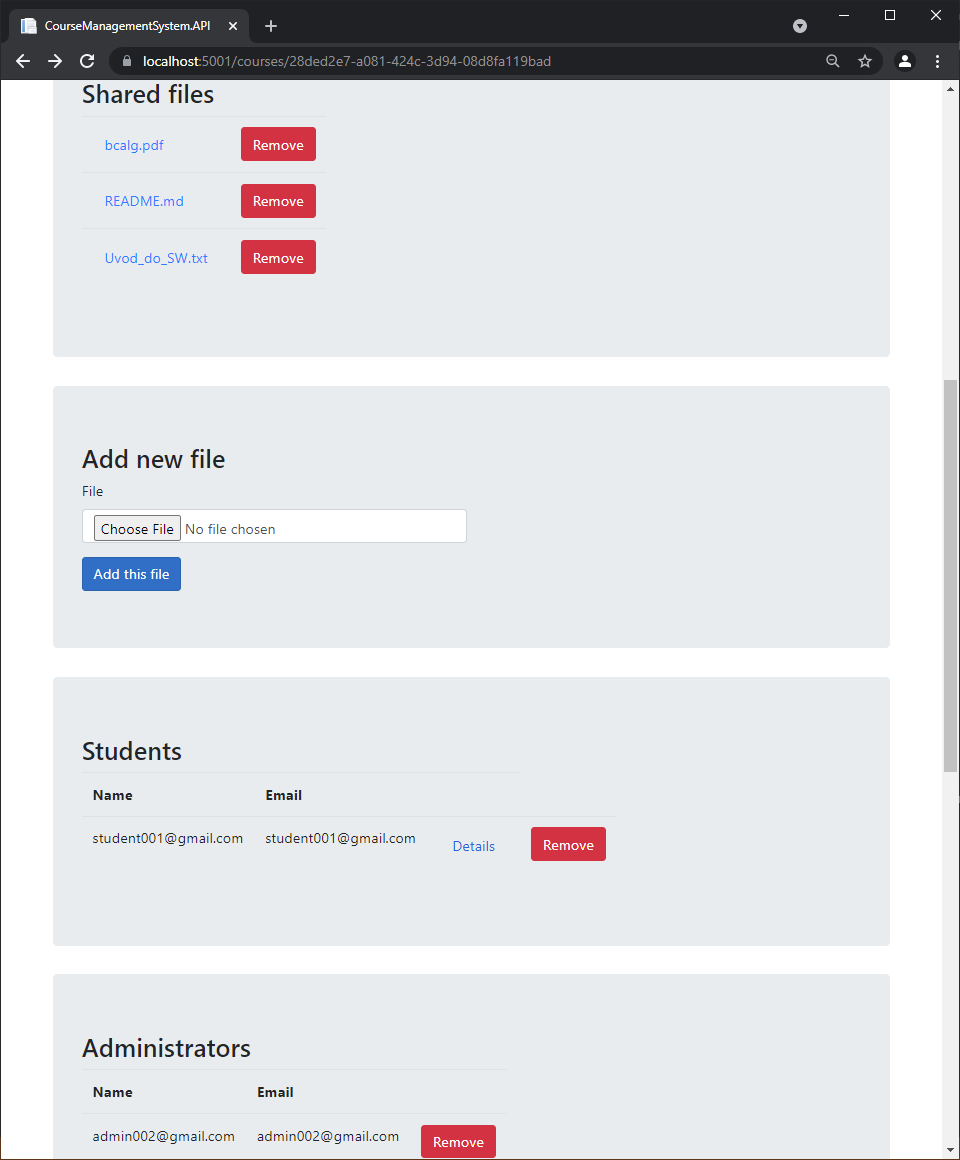
\includegraphics[width=\textwidth]{components_UI.PNG}
	\caption{Příklad UI s využitím komponent}
	\label{fig:Components}
\end{figure}

Na obrázku \ref{fig:Components} vidíme část UI s využitím několika komponent. Každá komponenta reprezentuje jeden logický celek uživatelského rozhraní. Konkrétně v uvedeném příkladu máme tyto komponenty:

\begin{itemize}
	\item Komponenta se seznamem souborů + formulářem pro přidání souboru
	\item Seznam studentů
	\item Seznam administrátorů
\end{itemize}

Šablona komponenty je typicky napsaná v HTML, zatímco backend je naprogramován v jazyce Typescript. 

\lstset{style=typescript}

\begin{program}
	\begin{lstlisting}
	@Component({
		selector: 'app-student-list',
		templateUrl: './student-list.component.html',
		styleUrls: ['./student-list.component.css']
	})
	export class StudentListComponent implements OnInit {
	
		@Input()
		private courseId: string;
		
		/**
		* list of students
		*/
		public students: CourseMemberOrAdminVM[] = [];
		
		private readonly courseService: CourseService;
		...
		
		constructor(courseService: CourseService, ...) {
			this.courseService = courseService;
			...
		}
		
		ngOnInit() {
			this.reloadData();
		}
		
		/**
		* reload student list
		* @private
		*/
		private reloadData(): void {
			this.courseService.getAllMembers(this.courseId)
			.subscribe(result => {
				this.students = result;
			});
		}
		
		...
	\end{lstlisting}
	\caption{Ukázka backendu komponenty}
	\label{ComponentBackend}
\end{program}

Na příkladu (Kód \ref{ComponentBackend}) vidíme, že backend komponenty je klasická Typescript třída označená anotací \textit{@Component}. U anotace je zároveň uvedený selektor, což je jméno HTML elementu, který slouží k vykreslení komponenty, a umístění souboru se šablonou a CSS styly.

Komponenty typicky používají služby k získání dat z API, podobně jako v příkladu. Můžeme si všimnout, že právě zde probíhá volání metody \textit{subscribe}, pomocí které v tomto případě data uložíme do proměnné \textit{students}.

Veřejné položky (například pole \textit{students}) jsou pak dostupné v HTML šabloně. Některé položky (například \textit{courseId}) jsou označené anotací \textit{@Input()}, která označuje parametry šablony.

Pro ilustraci uvedeme také šablonu komponenty (Kód \ref{ComponentTemplate}).

\lstset{style=html}

\begin{program}
	\begin{lstlisting}
	<div class="jumbotron">
		<h3>Students</h3>
		<table class="table table-striped table-responsive">
			<tr>
				<th>Username</th>
				<th></th>
				<th></th>
			</tr>
			<tr *ngFor="let person of students">
				<td class="align-middle">
					{{person.name}}
				</td>
				<td>
					<a class="btn btn-link" (click)=
						"pageNavigator.
						navigateToStudentDetail(
							person.id
						)">
						Details
					</a>
				</td>
				<td>
					<button class="btn btn-danger" 
					(click)="removeMember(person)">
						Remove
					</button>
				</td>
			</tr>
		</table>
		<div class="my-2">
			<div>
				<button class="btn btn-info" (click)="pageNavigator.
					navigateToCourseEnrollmentRequests(
						courseId
					)">
					Enrollment requests
				</button>
			</div>
		</div>
	</div>
	\end{lstlisting}
	\caption{Ukázka šablony komponenty}
	\label{ComponentTemplate}
\end{program}

Toto je šablona, která přísluší komponentě \textit{StudentListComponent}, jenž slouží k zobrazení členů kurzu. Vidíme, že se jedná o klasické HTML, do kterého můžeme vkládat proměnné z backend části komponenty.
Mezi složené závorky vložíme proměnnou, jež chceme vypsat, a framework Angular se sám postará o dosazení příslušné hodnoty.

Můžeme si všimnout atributu \textit{*ngFor} u elementu \textit{<tr>}. Takto definujeme, že v tabulce bude pro každého studenta samostatný řádek.
Na každém řádku následně vypíšeme jméno, email a odkaz na detail studenta.

\vspace{\baselineskip}

V šablonách komponent můžeme také vykreslovat jiné šablony.

\begin{lstlisting}
<app-test-list [courseId]="courseId" [isCourseAdmin]="isCourseAdmin"></app-test-list>
<app-file-list [courseId]="courseId" [isCourseAdmin]="isCourseAdmin"></app-file-list>
<app-student-list *ngIf="isCourseAdmin" [courseId]="courseId"></app-student-list>
...
\end{lstlisting}

Na tomto příkladu vidíme kus kódu ze šablony komponenty \textit{CourseDetailsComponent}, která slouží k zobrazení informací o daném kurzu. Šablona tedy na daném místě vykreslí příslušné šablony (v tomto případě komponenty se seznamy testů, souborů a studentů).

Při volání šablon můžeme také uvést parametry (například parametr \textit{courseId} v šabloně dané selektorem \textit{app-test-list}). Tato hodnota se pak uloží do příslušné položky, která je označená anotací \textit{@Input()}, v dané komponentě. To znamená, že komponenta se selektorem \textit{app-test-list} má položku \textit{courseId}, která je označená anotací \textit{@Input()}. Pro lepší představu ještě uvedeme kód \ref{ComponentWithParam}, na kterém se nachází třída s komponentou.

\lstset{style=typescript}

\begin{program}
	\begin{lstlisting}
	@Component({
		selector: 'app-test-list',
		templateUrl: './test-list.component.html',
		styleUrls: ['./test-list.component.css']
	})
	export class TestListComponent implements OnInit, OnChanges {
	
		@Input()
		public courseId: string;
		...
	}
	\end{lstlisting}
	\caption{Ukázka komponenty s parametrem}
	\label{ComponentWithParam}
\end{program}

\vspace{\baselineskip}

Vzhled stránky se u některých komponent liší podle toho, v jaké je uživateli roli. Můžeme tedy mít komponenty nebo kusy HTML kódu, které se zobrazují například pouze administrátorům daného kurzu.
Toto ve většině případů zajistíme pomocí proměnné, podle které poznáme, jestli je aktuální uživatel administrátor.
Pomocí atributu \textit{*ngIf} pak zajistíme, že daná část kódu se zobrazí pouze vybraným uživatelům.

\begin{lstlisting}
<app-student-list *ngIf="isCourseAdmin" [courseId]="courseId"></app-student-list>
\end{lstlisting}

V tomto příkladu používáme proměnnou \textit{isCourseAdmin}, a pomocí atributu \textit{*ngIf} zajistíme, že komponenta určená selektorem \textit{app-student-list} se zobrazí pouze administrátorům daného kurzu. 

\vspace{\baselineskip}

V komponentách také poměrně často využíváme obousměrný data binding, který je součástí frameworku Angular. Jedná se o techniku, která umožňuje synchronizaci dat mezi HTML a Typescript objekty.

Pokud tedy změníme data v HTML (například pole formuláře), framework se postará o změnu dat příslušné proměnné v backendu komponenty. Naopak, pokud dojde ke změně hodnoty dané proměnné, pak se framework postará o změnu HTML (například upraví text v poli formuláře).

Obousměrný data binding používáme typicky ve formulářích, podobně jako v následujícím příkladu.

\lstset{style=typescript}
\begin{lstlisting}
export class AddGradeComponent implements OnInit {
	/**
	* grade that will be added to the student
	*/
	public gradeToAdd: AddGradeVM;
	...
}
\end{lstlisting}

Toto je komponenta, která slouží k přidávání známek. 

\lstset{style=html}
\begin{program}
	\begin{lstlisting}
	...
	<div class="form-group col-md-2">
		<label for="addGradeForm_Value">Score in %</label>
		<input type="number" min="0" class="form-control" name="value" id="addGradeForm_Value" required
		[(ngModel)]="gradeToAdd.percentualValue">
	</div>
	<div class="form-group col-md-2">
		<label for="addGradeForm_Weight">Weight</label>
		<input type="number" min="0" class="form-control" name="weight" id="addGradeForm_Weight" required
		[(ngModel)]="gradeToAdd.weight">
	</div>
	...
	\end{lstlisting}
	\caption{Ukázka šablony, která používá obousměrný data binding}
	\label{TemplateTwoWayBinding}
\end{program}

V šabloně pak máme (mimo jiné) políčka formuláře pro procentuální hodnotu a váhu známky.
Pomocí atributu \textit{[(ngModel)]} nastavíme proměnnou pro data binding (Kód \ref{TemplateTwoWayBinding}). 

Pokud tedy například změníme ve formuláři váhu známky, dojde automaticky ke změně hodnoty \textit{gradeToAdd.weight}. Podobně, pokud dojde v kódu ke změně hodnoty proměnné \textit{gradeToAdd.weight}, framework automaticky upraví hodnotu ve formuláři.

Ke stylování elementů používáme framework Bootstrap, který nám také zajišťuje, že uživatelské rozhraní aplikace je responzivní.

\subsection{Routing}

Frontend část aplikace mimo jiné provádí také routing. Samotný router je součástí frameworku Angular, nicméně potřebujeme nějak nakonfigurovat, jaká komponenta se zobrazí při dotazu na danou URL.

Tato konfigurace se nachází v souboru app.module.ts.
\lstset{style=typescript}
\begin{lstlisting}
RouterModule.forRoot([
	{path: '', component: HomeComponent, pathMatch: 'full'},
	{path: 'students/:id', component: StudentDetailComponent},
	{path: 'courses', component: CourseListComponent},
	...
\end{lstlisting}

V konfiguraci máme vždy uvedenou cestu, a komponentu, která se zobrazí.
Vidíme tedy, že na výchozí stránce bude komponenta \textit{HomeComponent}. 
Druhý řádek nám říká, že při zadání URL \textit{http://host/students/id}, kde \textit{id} je parametr, se zobrazí komponenta \textit{StudentDetailComponent}. K parametru \textit{id} se poté můžeme dostat v komponentě.
Poslední řádek definuje, že na stránce \textit{http://host/courses} se zobrazí \textit{CourseListComponent}.

K navigaci mezi stránkami nepoužíváme přímo vestavěný router, ale pomocnou třídu \textit{PageNavigator}, která se nachází ve složce \textit{src/app/tools}. Tato třída obsahuje referenci na třídu \textit{Router} a metody, které slouží k navigaci na jednotlivé stránky. Pro každou stránku máme tedy jednu navigační metodu.

Na následujícím příkladu vidíme kód metody \textit{navigateToCourseDetail}, která slouží k navigaci na stránku s detaily daného kurzu.
\begin{lstlisting}
/**
* navigate to the page with course details
* @param courseId identifier of the course
*/
public navigateToCourseDetail(courseId: string): void {
	this.router.navigate(['/courses', courseId]).then(this.scrollToTop);
}
\end{lstlisting}


\section{Další vybrané problémy}

\subsection{ViewModely x Databázové entity}

Můžeme si všimnout, že v kódu používáme různé objekty pro ViewModely a databázové entity. 
Na následujícím příkladu můžeme vidět největší rozdíly mezi těmito objekty.

\lstset{style=sharpc}

\begin{program}
	\begin{lstlisting}
	public class TestSubmissionAnswer : IGuidIdObject
	{	
		/// <summary>
		/// question which is answered
		/// </summary>
		[Required]
		public TestQuestion Question { get; set; }
		
		/// <summary>
		/// submitted text of the answer
		/// </summary>
		public string Text { get; set; }
		
		/// <summary>
		/// points obtained for the answer
		/// </summary>
		public int Points { get; set; }
		...
	}
	\end{lstlisting}
	\caption{Databázová entita \textit{TestSubmissionAnswer}}
	\label{DbEntityTestSubmissionAnswer}
\end{program}

\begin{program}
	\begin{lstlisting}
	public class SubmissionAnswerVM
	{	
		/// <summary>
		/// number of question that this answer belongs to
		/// </summary>
		[PositiveIntValue]
		public int QuestionNumber { get; set; }
		
		/// <summary>
		/// text of the question
		/// </summary>
		[RequiredWithDefaultErrorMessage]
		public string QuestionText { get; set; }
		
		/// <summary>
		/// answer submitted by the student
		/// </summary>
		public string AnswerText { get; set; }
		...
	}
	\end{lstlisting}
	\caption{ViewModel \textit{SubmissionAnswerVM}}
	\label{ViewmodelTestSubmissionAnswer}
\end{program}

Na ukázkách kódu \ref{DbEntityTestSubmissionAnswer} a \ref{ViewmodelTestSubmissionAnswer} vidíme databázovou entitu \textit{TestSubmissionAnswer} a ViewModel \textit{SubmissionAnswerVM}, oba typy reprezentují odpověď studenta na danou otázku.
Vidíme, že v tomto případě ViewModel obsahuje vlastnosti převzaté z více databázových entit, což je velmi častá situace. Vlastnosti \textit{QuestionNumber} a \textit{QuestionText} jsou převzaté z entity \textit{TestQuestion}, naopak vlastnost \textit{AnswerText} je z entity \textit{TestSubmissionAnswer}.

Některé jiné ViewModely naopak obsahují jen vybrané vlastnosti příslušných databázových entit, ostatní data jsou v daném kontextu zbytečná.

Z toho vyplývá, že nemůžeme použít instance stejné třídy pro tyto typy objektů.

Pokud bychom se rozhodli použít dědičnost (tedy např. ViewModel by dědil z databázové entity, příp. naopak), narazili bychom na problém s atributy.
Téměř všechny databázové entity totiž obsahují atributy, které slouží ke konfiguraci databázových tabulek, naopak ViewModely obsahují atributy pro validaci. 

Vzhledem k výše uvedeným argumentům tedy používáme různé objekty.


\subsection{ViewModely v serverové i klientské části}

V kapitolách \ref{serverVM} a \ref{clientVM} můžeme vidět, že ViewModely se nachází jak v serverové, tak i v klientské části aplikace. 

Tyto ViewModely jsou shodné (obsahují tedy stejné položky), akorát jsou zapsané v jiném jazyce. ViewModely v serverové části navíc často obsahují atributy, které slouží k validaci dat.

Typ položek je ve většině případů stejný, někdy se ovšem může lišit. To je většinou z toho důvodu, že neexistují typy, které si v jazycích C\# a Typescript přesně odpovídají.
Například jazyk Typescript používá pro všechna čísla typ \textit{number}, zatímco v jazyce C\# můžeme použít několik typů. 
Pro celá čísla používáme např. typy \textit{int} a \textit{long}, pro desetinná čísla \textit{float} či \textit{double}.

Toto řešení je nutné, abychom mohli s ViewModely pracovat v obou částech aplikace.